Graphs are fundamental data structures in many applications, such as computer networks, recommendation systems, and circuit design. In recent years, a number of high performance graph processing frameworks have emerged. State-of-the-art frameworks include Gunrock \cite{wang2016gunrock}, Hornet \cite{busato2018hornet}, Ligra \cite{shun2013ligra}, and Galois \cite{nguyen2013lightweight}.\ignore{These frameworks have demonstrated efficient computation on billion-scale graphs.} Their emphasis lies in accelerating graph analytics tasks by providing high-performance kernels tailored to diverse datasets.

Unfortunately, loading graph data is a significant bottleneck in such frameworks. In fact, the cost of loading data can dominate the overall processing time --- especially as computational capabilities continue to improve\ignore{\cite{gabert2021pigo}}. Gabert and Çatalyürek \cite{gabert2021pigo} observe that\ignore{even on high-performance shared-memory graph systems running billion-scale graphs,} reading the graph from file systems, on such frameworks, takes multiple orders of magnitude longer than running the computational kernel. This slowdown not only causes a disconnect for end users and a loss of productivity for researchers\ignore{/developers}, but also increases the system/cloud usage charges. Fast loading of graphs is thus, crucial\ignore{for minimizing the time it takes to start processing and analyzing the graph data}.\ignore{This motivates us to work on efficient IO techniques. These not only improve response time, but also help lower system / cloud usage charges.}

In modern frameworks like Gunrock, loading graph data from ASCII-based file formats, specifically using the Coordinate (COO) format, is a major bottleneck. To load the graph as an Edgelist, these frameworks typically follow a sequential process of opening the input file, reading the entries one by one, and inserting them into an array. If the goal is to access the graph in the Compressed Sparse Row (CSR) format, which is often the case --- due to its storage efficiency and locality benefits, additional steps are required. These include computing the out-degrees of vertices from the Edgelist, performing prefix sum to determine the offsets of outgoing edges in the CSR representation, and then populating the CSR arrays with edges from the Edgelist. All these operations are carried out sequentially, contributing to the overall loading time.

Many graph processing frameworks\ignore{have showcased efficient computation on large-scale graphs, they}, thus, still rely on sequential I/O. This is likely due to the belief that I/O devices tend to be slow (relative to the CPU), and that achieving parallel I/O necessitates specialized systems.\ignore{Graph and matrix I/O times are seldom reported in the literature.} However, modern IO devices are fast, and implementing only sequential I/O fails to exploit the capabilities of modern Hard Disk Drives (HDDs), Redundant Array of Independent Disks (RAID) controllers, and Non-Volatile Memory (NVM) \cite{gabert2021pigo}. A number of disk-based out-of-memory graph processing systems/frameworks\ignore{\cite{zhu2015gridgraph, cheng2015venus, chi2016nxgraph, ai2017squeezing, ma2017garaph, maass2017mosaic, wu2018redio, ai2018clip, jun2018grafboost, zhang2018wonderland}} \cite{kyrola2012graphchi, han2013turbograph, roy2013x, najeebullah2014bishard, lin2014mmap, zheng2015flashgraph, wang2021scaleg} focus on loading large graphs stored in binary formats. However, a majority of graph datasets exist in serialized human-readable data exchange formats.\ignore{To address this, our focus lies on efficiently loading graphs stored in plain text formats.}

To address these challenges, Gabert and Çatalyürek introduce PIGO \cite{gabert2021pigo}, a header-only, dependency-free C++11 parallel graph loader that supports loading graphs in memory as Edgelists or CSR. PIGO leverages memory mapping, a mechanism that maps a file or part of a file into the virtual memory space\ignore{so that files on the disk can be accessed as if they were in memory} \cite{lin2014mmap}, to optimize file reading. This eliminates the need for repeated system calls, resulting in reduced context-switch overhead and improved efficiency, particularly if the kernel\ignore{accurately} predicts the accessed pages ahead of time.

However, we have identified a few issues with PIGO. Firstly, when reading entries from the input file, PIGO divides the file length equally among threads, potentially leading to slower overall performance as faster threads wait for slower ones. Secondly, PIGO utilizes a two-pass approach for loading graphs into memory as Edgelists, which involves first counting newlines to determine the number of edges and associated offsets for each thread, and then parsing and populating the Edgelist. This method is less efficient compared to a single-pass approach. This method is inefficient compared to a single-pass approach. When converting the Edgelist to a CSR representation, PIGO globally computes vertex degrees using atomics, uses it compute the offsets array of the global CSR, and iterates through the Edgelist to atomically populate the targets array of the global CSR. This global computation of vertex degrees, and directly operating on the shared CSR can lead to high contention between threads. Further, PIGO populates the targets array of the CSR with static load balancing, potentially leading to load imbalances among threads. Finally, when reading Matrix Market (MTX) files, a format commonly used for storing sparse graphs/matrices, PIGO disregards specified attributes, resulting in lower reported runtimes for symmetric graphs (the authors plan to address this\ignore{in the future}).

In this technical report, we propose GVEL\footnote{\url{https://github.com/puzzlef/graph-csr-openmp}}. Similar to PIGO, it employs memory mapping and parallelization to optimize graph loading. However, GVEL improves upon PIGO by efficiently processing the graph as per-thread Edgelists in a single pass through overallocation of memory via memory mapping. Note that this does not waste memory, as untouched pages are never mapped to DRAM. To convert the per-thead Edgelists to CSR, GVEL computes four independent sets of vertex degrees (which, when summed up for each vertex, represents the global degree of each vertex), and uses it to generate the global CSR representation in a novel staged manner. It does this by first obtaining $4$ independent sets of CSRs, and then combining them together, in parallel, to form a global CSR. This minimizes the contention between threads\ignore{, which we observe to be a significant bottleneck for converting an Edgelist to CSR}. These techniques allow GVEL to achieve a $2.6\times$ speedup over PIGO for loading graphs into memory as Edgelists, and a speedup of $1.8\times$ for loading graphs into memory as CSRs (i.e., reading the graph as Edgelist and then converting it to CSR). Our techniques may also be used to convert in-memory Edgelists (an update friendly data structure), to a CSR (a space efficient and locality efficient data structure).
\ignore{Our techniques may also be useful for converting COO to CSR on the fly on parallel devices. This is important since CSR is an efficient data structure, while COO is easy to update. Per-thread COOs are not needed - we can use single COO and split it unto parts for each thread to process.}




% x Why do HP G frameworks load graphs slowly?
% x A quick glimpse of how they do it.
% x Why do the persist with sequential IO? (Modern IO is fast)
% x What are the HP IO interfaces? (MMAP)
% x Which graphs frameworks make use of mmap? (external memory frameworks)
% x What do they focus on? (binary graph formats)
% x Why is fast loading of serialized formats important? (human readable data exchange format)
% x What have Gabert et al. done in PIGO?
% x How do we improve upon it? (link to code)

% - Measure EL, CSR, EL + CSR ...
% - Details of NVME, as much as possible.
% - Indirect comparison with Ligra, GAPbs, and Galois (PIGO).
% - Details of other graphs processing frameworks, and the above
% -- cugraph
% -- networkit
% -- igraph?
% -- gunrock
% -- hornet
% -- graphblast

% - adjust csr partitions
% - adjust csr partitions (convert csr only)
% - adjust block size
% - read EL, convert CSR split on graphs

% - Why fast graph loading is important?
% - Extremely high cost of loading compared to computation.
% - An issue with even popular graph processing frameworks.
% - Modern IO is fast (compared to CPU performance).
% - Storage capacities increasing, bandwidth is high, CPUs as not as fast as they used to be.
% - Common graph file formats (COO, MTX).
% - Common memory storage formats (Edgelist, CSR).
% - Work presented in this paper.




%% - Use --- for a dash.
%% - Use ``camera-ready'' for quotes.
%% - Use {\itshape very} or \textit{very} for italicized text.
%% - Use \verb|acmart| or {\verb|acmart|} for mono-spaced text.
%% - Use \url{https://capitalizemytitle.com/} for URLs.
%% - Use {\bfseries Do not modify this document.} for important boldface details.
%% - Use \ref{fig:name} for referencing.

%% For a block of pre-formatted text: 
% \begin{verbatim}
%   \renewcommand{\shortauthors}{McCartney, et al.}
% \end{verbatim}

%% For a list of items:
% \begin{itemize}
% \item the ``ACM Reference Format'' text on the first page.
% \item the ``rights management'' text on the first page.
% \item the conference information in the page header(s).
% \end{itemize}

%% For a table:
% \begin{table}
%   \caption{Frequency of Special Characters}
%   \label{tab:freq}
%   \begin{tabular}{ccl}
%     \toprule
%     Non-English or Math&Frequency&Comments\\
%     \midrule
%     \O & 1 in 1,000& For Swedish names\\
%     $\pi$ & 1 in 5& Common in math\\
%     \$ & 4 in 5 & Used in business\\
%     $\Psi^2_1$ & 1 in 40,000& Unexplained usage\\
%   \bottomrule
% \end{tabular}
% \end{table}

%% For a full-width table:
% \begin{table*}
%   \caption{Some Typical Commands}
%   \label{tab:commands}
%   \begin{tabular}{ccl}
%     \toprule
%     Command &A Number & Comments\\
%     \midrule
%     \texttt{{\char'134}author} & 100& Author \\
%     \texttt{{\char'134}table}& 300 & For tables\\
%     \texttt{{\char'134}table*}& 400& For wider tables\\
%     \bottomrule
%   \end{tabular}
% \end{table*}


%% For inline math:
% \begin{math}
%   \lim_{n\rightarrow \infty}x=0
% \end{math},

%% For a numbered equation:
% \begin{equation}
%   \lim_{n\rightarrow \infty}x=0
% \end{equation}

%% For an unnumbered equation:
% \begin{displaymath}
%   \sum_{i=0}^{\infty} x + 1
% \end{displaymath}

%% For a figure:
% \begin{figure}[h]
%   \centering
%   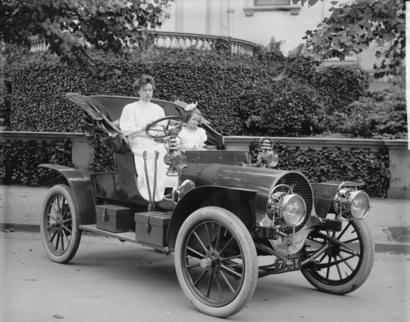
\includegraphics[width=\linewidth]{inc/sample-franklin}
%   \caption{1907 Franklin Model D roadster. Photograph by Harris \&
%     Ewing, Inc. [Public domain], via Wikimedia
%     Commons. (\url{https://goo.gl/VLCRBB}).}
%   \Description{A woman and a girl in white dresses sit in an open car.}
% \end{figure}

%% For a teaser figure.
% \begin{teaserfigure}
%   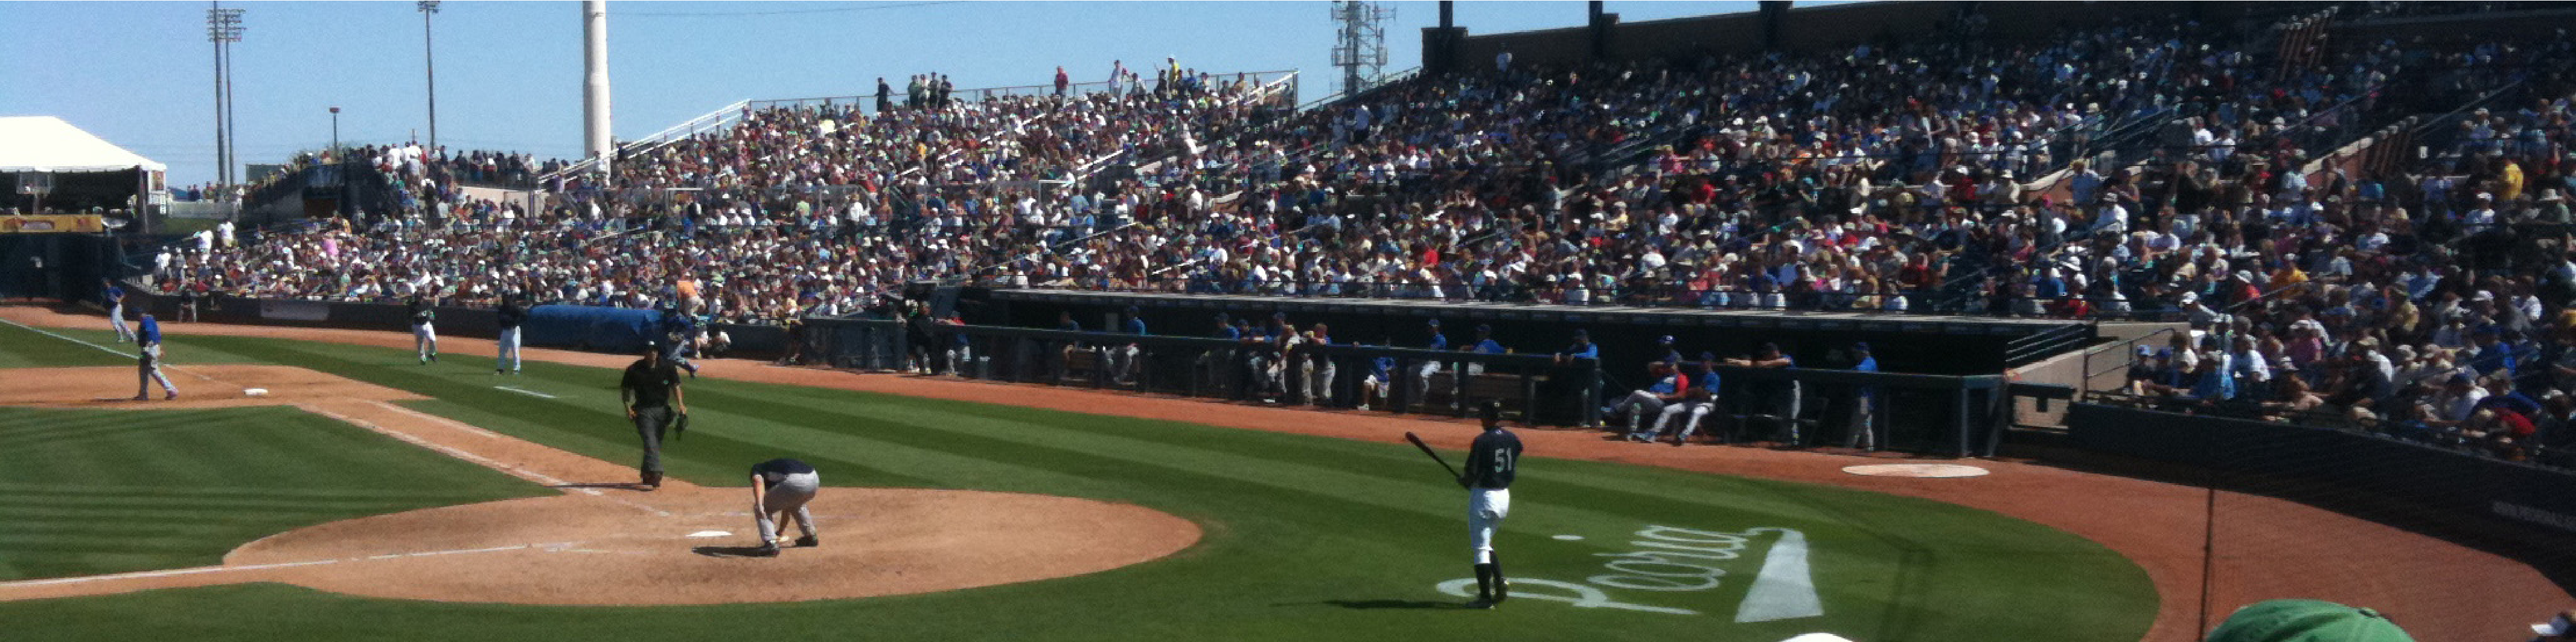
\includegraphics[width=\textwidth]{sampleteaser}
%   \caption{figure caption}
%   \Description{figure description}
% \end{teaserfigure}
